%%
%% This is file `sample-sigconf.tex',
%% generated with the docstrip utility.
%%
%% The original source files were:
%%
%% samples.dtx  (with options: `all,proceedings,bibtex,sigconf')
%%
%% IMPORTANT NOTICE:
%%
%% For the copyright see the source file.
%%
%% Any modified versions of this file must be renamed
%% with new filenames distinct from sample-sigconf.tex.
%%
%% For distribution of the original source see the terms
%% for copying and modification in the file samples.dtx.
%%
%% This generated file may be distributed as long as the
%% original source files, as listed above, are part of the
%% same distribution. (The sources need not necessarily be
%% in the same archive or directory.)
%%
%%
%% Commands for TeXCount
%TC:macro~\cite [option:text,text]
%TC:macro~\citep [option:text,text]
%TC:macro~\citet [option:text,text]
%TC:envir table 0 1
%TC:envir table* 0 1
%TC:envir tabular [ignore] word
%TC:envir displaymath 0 word
%TC:envir math 0 word
%TC:envir comment 0 0
%%
%% The first command in your LaTeX source must be the \documentclass
%% command.
%%
%% For submission and review of your manuscript please change the
%% command to \documentclass[manuscript, screen, review]{acmart}.

\documentclass[acmsmall, manuscript, screen, review, anonymous]{acmart}
%%
%% \BibTeX command to typeset BibTeX logo in the docs
\AtBeginDocument{%
  \providecommand\BibTeX{{%
    Bib\TeX}}}

\setcopyright{acmlicensed}
\copyrightyear{2025}
\acmYear{2025}
\acmDOI{XXXXXXX.XXXXXXX}
\acmConference[SPAA '25]{37th ACM Symposium on Parallelism in Algorithms and Architectures}{July 28--August 1,
  2025}{Portland, OR, USA}
\acmISBN{978-1-4503-XXXX-X/18/06}

\usepackage[ruled,vlined]{algorithm2e}
\SetKwInput{KwGlobalIn}{Global Mem Input}
\SetKwInput{KwSharedIn}{Shared Mem Input}
\SetKwInput{KwSharedOut}{Shared Mem Output}
\SetKwInput{KwGlobalOut}{Global Mem Output}
\SetKwInput{KwConstants}{Constants}

\usepackage{amsmath}
\usepackage{mathtools}
\usepackage{listings}
\usepackage{subcaption}
\usepackage{makecell}
\newcommand{\thomas}[1]{{\footnotesize\color{orange}[Thomas: #1]}}
\newcommand{\john}[1]{{\footnotesize\color{cyan}[John: #1]}}
\newcommand{\raph}[1]{{\footnotesize\color{magenta}[Raph: #1]}}

\begin{document}

\title{Decoupled Fallback: A Portable Single-Pass GPU Scan}

\author{Thomas Smith}
\affiliation{%
  \institution{Google}
  \country{USA}}

\author{Raph Levien}
\affiliation{%
  \institution{Google}
  \country{USA}
}

\author{John D. Owens}
\affiliation{%
  \institution{University of California, Davis}
  \country{USA}}
\additionalaffiliation{%
  \institution{Google}
  \country{USA}
}

\renewcommand{\shortauthors}{Smith et al.}

\begin{abstract}
  We present \emph{Decoupled Fallback}, a method that enables single-pass \emph{Chained Scans} to run on hardware without \emph{forward-progress guarantees} (FPG) while avoiding deadlock. Additionally, we introduce a tile state representation for \emph{Chained Scans} that does not rely on 64-bit atomics or memory barriers for correctness, along with a subgroup-size-agnostic intra-workgroup implementation. On FPG-lacking devices---Apple M1 Max and M3---\emph{Decoupled Fallback} achieves near-\emph{Memcpy} speeds for inclusive prefix sum in WGPU and realizes the full theoretically expected 50\% speedup over the slower \emph{Reduce-then-Scan} approach. We further demonstrate the resilience of \emph{Decoupled Fallback} against \emph{unfair} schedulers by simulating blocking at rates of up to 50\%, showing that it maintains superior performance over \emph{Reduce-then-Scan} even under extreme contention.
\end{abstract}

\begin{CCSXML}
  <ccs2012>
  <concept>
  <concept_id>00000000.0000000.0000000</concept_id>
  <concept_desc>Do Not Use This Code, Generate the Correct Terms for Your Paper</concept_desc>
  <concept_significance>500</concept_significance>
  </concept>
  <concept>
  <concept_id>00000000.00000000.00000000</concept_id>
  <concept_desc>Do Not Use This Code, Generate the Correct Terms for Your Paper</concept_desc>
  <concept_significance>300</concept_significance>
  </concept>
  <concept>
  <concept_id>00000000.00000000.00000000</concept_id>
  <concept_desc>Do Not Use This Code, Generate the Correct Terms for Your Paper</concept_desc>
  <concept_significance>100</concept_significance>
  </concept>
  <concept>
  <concept_id>00000000.00000000.00000000</concept_id>
  <concept_desc>Do Not Use This Code, Generate the Correct Terms for Your Paper</concept_desc>
  <concept_significance>100</concept_significance>
  </concept>
  </ccs2012>
\end{CCSXML}

\ccsdesc[500]{Do Not Use This Code~Generate the Correct Terms for Your Paper}
\ccsdesc[300]{Do Not Use This Code~Generate the Correct Terms for Your Paper}
\ccsdesc{Do Not Use This Code~Generate the Correct Terms for Your Paper}
\ccsdesc[100]{Do Not Use This Code~Generate the Correct Terms for Your Paper}

\keywords{Do, Not, Us, This, Code, Put, the, Correct, Terms, for,
  Your, Paper}

%\received{?}
%\received[revised]{?}
%\received[accepted]{?}

\maketitle

\section{Introduction}
Scan is one of the most ubiquitous operations in GPU computing, with applications in sorting~\cite{adinets2022onesweepfastersignificantdigit}, sparse matrix operations~\cite{BellGarland2009}, and more. The current state-of-the-art prefix scan algorithm, Merrill and Garland's \emph{Decoupled Lookback}, achieves near-ideal performance on NVIDIA hardware via CUDA by leveraging the \emph{Chained Scan} architecture. This approach hybridizes serial and parallel strategies to read and write each element exactly once, achieving the theoretical minimum global memory movement of $O(2n)$. \emph{Chained Scans} that fully saturate device memory bandwidth reach the \emph{Speed of Light} (SOL) performance limit---the theoretical maximum throughput constrained by the physical limits of the device. However, \emph{Decoupled Lookback} relies on architectural and language-specific guarantees provided by the NVIDIA ecosystem, most notably a device scheduler property known as a \emph{forward-progress guarantee}; without this guarantee, it risks indefinite starvation and will never complete. In practice, it is easy to demonstrate this behavior.

As the compute capabilities of major graphics APIs---Vulkan, Direct3D, and Metal---have grown, there has been increasing interest in adapting \emph{Decoupled Lookback} beyond CUDA for broader adoption in real-time graphics and GPU computing. However, portable implementation is constrained by both hardware and API limitations. In terms of hardware, some GPU schedulers—most notably Apple's M series and ARM—lack forward-progress guarantees, and subgroup sizes vary across architectures. In terms of API design, the absence of 64-bit atomic operations and explicit memory barriers further complicates implementation, as both are integral to \emph{Decoupled Lookback}.

This work is guided by two main goals. (1) \textbf{Portability:} We aim to develop a scan implementation that retains the benefits of the \emph{Chained Scan} architecture while being suitable for a diverse range of hardware vendors and architectures, including those without forward-progress guarantees (FPG) or support for 64-bit atomics. \textbf{Performance:} We aim for near speed-of-light execution to the greatest extent possible allowed by the underlying hardware and programming model.

However, certain aspects fall outside the scope of this work. \textbf{Performance guarantees} are not universally attainable, as not all architectures offer atomic operations that are sufficiently fast or scheduling models that are sufficiently fair to attain speed-of-light performance. \textbf{Subgroup divergence} is another challenge we acknowledge but do not address directly, as shading languages do not provide explicit divergence control like CUDA's subgroup masking mechanisms. Lastly, we do not investigate alternative $O(2n)$ scan architectures beyond \emph{Chained Scan}.

We present \emph{Decoupled Fallback}, a fully portable prefix scan capable of achieving speed-of-light performance without requiring forward-progress guarantees (FPG). Our implementation is designed for compatibility with shading languages, making it suitable for modern graphics APIs and implemented in the WebGPU Shading Language (WGSL)\@. \john{I don't love ``compatibility with shading languages'' but then we name a single shading language. Instead, maybe something like ``Our implementation targets portability across modern GPU hardware and software platforms'', that sort of thing?} Our method incorporates a novel tile state representation that eliminates reliance on 64-bit atomics or memory barriers while maintaining correctness, along with a subgroup-size-agnostic intra-workgroup implementation that enables subgroup acceleration across all architectures.

\section{Background}
\subsection{Virtualization and Scheduling in the GPU programming model}
Contemporary GPUs are hierarchically organized, massively parallel processors designed to prioritize throughput over latency. As comprehensive descriptions of the GPU programming model~\cite{10.1145/1365490.1365500} already exist, we focus on the aspects most relevant to this work: scheduling and synchronization.

On GPU hardware, scheduling is divided into two levels: a \emph{workgroup} scheduler, which manages kernel launches and maps virtual processors, workgroups, to physical processors, \emph{multiprocessors}, and a \emph{subgroup} scheduler, responsible for selecting a subset of the currently \emph{occupant} subgroups on a multiprocessor for execution. The GPU programming model virtualizes processors to ensure GPU programs---\emph{kernels}---remain portable across hardware with differing physical resources. Effective virtualization requires \emph{oversubscription}, a programming paradigm where tasks are (over)partitioned in such a way that kernels request more virtual processors than are physically available. As a result, a single multiprocessor may host multiple workgroups simultaneously. However, as a consequence of virtualization, the developer relinquishes control over the order in which workgroups are launched, and once a workgroup begins execution on a multiprocessor, it must run to completion and cannot context-switch.

\subsubsection{Inter-Workgroup Barriers}
Parallel programs in general require synchronization between multiple threads (those that don't are considered embarrassingly parallel). A standard technique for synchronization is \emph{barriers.} GPUs provide a limited palette of barrier primitives. At the coarsest granularity, \emph{pipeline barriers} fully synchronize both control and memory between multiple kernel launches. However, pipeline barriers are extremely expensive and efficient algorithms strictly minimize their use. At a much finer granularity, \emph{workgroup barriers} provide reasonably efficient synchronization between the threads in a workgroup. However, synchronization between workgroups is more limited. Standard GPU programming environments provide no control barrier between workgroups.\footnote{CUDA recently introduced \emph{Thread Block Cluster} synchronization~\cite{NvidiaCudaGuide}, but it is almost certainly designed to operate within the \emph{Persistent Thread}~\cite{gupta2012} paradigm, rather than serving as a barrier across an unbounded launch.} The availability of a memory-only barrier varies across GPU environments; it is present in Direct3D and Vulkan, but was missing in versions of Metal prior to 3.2. Because of its non-portability, it is also absent from the WebGPU specification. Even when available, the use of such memory barriers causes performance issues as they are usually implemented as a full cache flush.

\subsubsection{Fairness and Progress}
Because multiple workgroups may reside on a single multiprocessor, two key issues arise at the subgroup scheduling level: \emph{fairness}---how evenly execution resources are distributed among subgroups---and \emph{progress guarantees}---ensuring that subgroups eventually make progress towards termination. However, the term ``fairness'' is used differently across the literature, leading to potential confusion. Sorensen et al.~\cite{sorensen2016,sorensen2018,sorensen2021}, whose work provides the most comprehensive taxonomy of progress models to date, use ``fairness'' specifically to describe differing levels of progress guarantees. In contrast, NVIDIA publications~\cite{4523358,Merrill2016} define ``fairness'' in terms of the distribution of execution resources among subgroups. In this work, we adopt NVIDIA's terminology.

\subsection{The Scan Primitive}%
\label{sec:the-scan-primitive}
The study of \emph{scan} (\emph{parallel prefix}) networks traces back to the design of carry-lookahead adder circuits and beyond~\cite{5219801,10.5555/1098666}. A scan is typically defined on a monoid \( M \), characterized by a binary reduction operator \( \oplus \) and an identity element \( \varepsilon \). The binary operator \( \oplus \) satisfies the closure property \( \forall a, b \in M, \ (a \oplus b) \in M \) and has an identity element \( \exists \varepsilon \in M, \ \forall a \in M, \ \varepsilon \oplus a = a \). To allow parallelization, \( \oplus \) must be associative, but it is not necessarily commutative, as demonstrated in structures like the \emph{bicyclic semigroup}~\cite{Clifford1961}\footnote{Despite its name, this is a monoid.} and Rabin-Karp's \emph{second fingerprinting method for string matching}~\cite[Section 6]{Karp:1987:ERP}. In a scan, the result at the \( n \)-th element is the reduction of the preceding subsequence of elements. If the subsequence includes the \( n \)-th element, it is called \emph{inclusive}; if it excludes the \( n \)-th element, it is called \emph{exclusive}. The most common scan type is the prefix sum, where \( \oplus \) is addition. For example:
\[
  x = [x_1, x_2, x_3, \dots, x_n] \ \ \ \ \ \ \ y = [1, 1, 1, 1, 1]
\]
\[
  \text{InclusiveScan}(x, \oplus) = [x_1, x_1 \oplus x_2, x_1 \oplus x_2 \oplus x_3, \dots, x_1 \oplus x_2 \oplus \cdots \oplus x_n]
\]
\[
  \text{InclusiveScan}(y, +) = [1, 2, 3, 4, 5]
\]
Due to its significance in circuits and as a fundamental algorithmic primitive, scan has been extensively studied in both electrical engineering and computer science. Harris~\cite{1292373} offers a taxonomy that relates depth, fanout, and wire tracks, while Hinze~\cite{10.1007/978-3-540-27764-4_11} develops an algebraic framework for scans. Snir~\cite{10.1016/0196-67748690003-9} proved that depth $d$ and size $s$ are related by $s + d \ge 2n - 2$, and Fich~\cite{10.1145/800061.808738} proved that among minimum depth scans Ladner-Fischer~\cite{10.1145/322217.322232} networks have optimal size. Blelloch~\cite{Blelloch:1989:SAP} adapted scan to the PRAM model and popularized its use as an algorithmic primitive. Finally, Merrill and Garland~\cite{Merrill2016} provide a review of GPU scan implementations, complementing earlier work by Merrill and Grimshaw~\cite{Merrill2009}.

\subsection{Evolution of Inter-Workgroup Scan Architectures}
Contemporary GPU scans depart from early PRAM-like scans~\cite{Horn, Hensley, Sengupta2006, Gress} by leveraging the GPU memory hierarchy, which consists of progressively faster but increasingly private tiers. Efficient scans integrate fine-grained intra-workgroup (\emph{local}) strategies in shared memory and registers with coarse-grained inter-workgroup (\emph{global}) strategies in global memory. Given their low arithmetic intensity, local scans are inherently memory-bound, as demonstrated by Merrill and Grimshaw~\cite{Merrill2009}. Consequently, recent scan optimizations have shifted toward refining global strategies, particularly inter-workgroup coordination and synchronization. This section reviews three key approaches---\emph{Scan-then-Propagate}, \emph{Reduce-then-Scan}, and \emph{Chained Scan}---analyzing their handling of inter-workgroup dependencies and efficiency in minimizing global memory access while maximizing bandwidth utilization.

\subsubsection{Scan-then-Propagate}
Introduced by Sengupta et al.~\cite{10.5555/1280094.1280110}, \emph{Scan-then-Propagate}~\cite{GPUGems3, Sengupta2011} extends intra-workgroup scans to large inputs by resolving inter-workgroup dependencies in three phases:
\begin{enumerate}
  \item \textbf{Intra-Workgroup (Local) Scan:}  Each workgroup performs an inclusive scan on its assigned work tile, storing local results and reductions in global memory.
  \item \textbf{Spine Scan:} The workgroup reductions, collectively forming the \emph{spine}, are gathered and scanned to compute the \emph{root}, resolving dependencies between work tiles. For large scans, this stage is an insignificant amount of work compared to the first and third.
  \item \textbf{Propagation:} Each workgroup retrieves its portion of the root and adds it to the local scan output.
\end{enumerate}
The absence of inter-workgroup barriers necessitates separate kernel launches and pipeline barriers for dependency resolution, naturally enforcing this structure. To accommodate arbitrarily large inputs, Sengupta et al.\ employ recursion, repeatedly applying the three-phase process until the spine fits within a single work tile. Thus, an input of size $n$ and a work tile of size $t$ results in a recursive depth of $\lceil \log_t n \rceil$, and $2\cdot\lceil \log_t n \rceil - 1$ kernel launches. Each recursive step $k$ processes $n/t^k$ tiles, leading to a total of $\sum_{k=1}^{\lceil \log_t n \rceil} n/t^k \approx (n - 1)/(t - 1)$ work tiles over all steps. Since each tile moves $4t$ data ($2t$ local scan, $2t$ propagation), the total global data movement is $O\left(\frac{4t(n - 1)}{t - 1}\right) = O(4n)$.

\subsubsection{Reduce-then-Scan}
If memory bandwidth resources are sufficiently scarce relative to compute, memory-bound algorithms like scan can profit by trading additional computation for reduced memory traffic. This trade-off led to a refinement of the \emph{Scan-then-Propagate} strategy called \emph{Reduce-then-Scan}~\cite{10.1145/1375527.1375559, Merrill2009, 10.1109/TPDS.2012.336, 10.5555/2031978.2032029}: by storing only the work tile reduction in global memory during the first phase and performing a redundant scan in the third, it eliminates $n$ global data movement while preserving the three-phase structure:
\begin{enumerate}
  \item \textbf{Work Tile Reduction:} Each workgroup performs a pure reduction on its work tile partition, posting the result to global memory.
  \item \textbf{Spine Scan:} The spine is scanned to produce the root.
  \item \textbf{Intra-Workgroup Scan and Propagation:} Each workgroup performs the local scan on the work tile, incorporating its portion of the root as it writes to global memory.
\end{enumerate}

Merrill and Grimshaw~\cite{Merrill2009} introduced \emph{workgroup raking} to reduce recursion overhead for arbitrarily large inputs. Instead of recursively reducing the spine, the input is partitioned among a fixed number of workgroups, $c$, where $c \geq o$, the total workgroup occupancy. This constrains the spine from a variable, potentially recursive structure to a fixed size $c$, ensuring a recursion depth of at most two. As a result, global memory movement for the spine scan is reduced from $O(n/t)$ to $O(2c)$, and kernel launches and pipeline barriers are limited to three, yielding a total global memory movement of $O(3n + 4c) = O(3n)$.

Breitbart~\cite{10.5555/2031978.2032029} applied Gupta et al.'s \emph{Persistent-Threads}~\cite{gupta2012} to scan, eliminating kernel launch overheads. Recognizing that raking naturally aligns with this paradigm, Breitbart's method statically \emph{discovers} the workgroup occupancy and launches exactly $o$ kernels. Since multiprocessors are not oversubscribed, workgroups persist for the entire kernel duration, enabling synchronization at an atomics-based inter-workgroup memory and control barrier without kernel launches or pipeline barriers. While global memory movement remains $O(3n)$, this consolidates the scan into a single kernel, minimizing launch and pipeline overheads.

\subsubsection{Chained Scan, StreamScan}
First introduced by Yan et al.~\cite{10.1145/2442516.2442539} in \emph{StreamScan}, the key innovation of the \emph{Chained Scan} architecture lies in its hybridization of parallel and serial strategies: achieving parallelism at the intra-workgroup level while minimizing global data movement through serial scan operations at the inter-workgroup level. Instead of using kernel launches and pipeline barriers as inter-workgroup synchronization points, \emph{Chained Scans} launch a single kernel that assigns work tiles in a serial order to workgroups, utilizing atomics and bit-packed status flags to ensure coherent views of data. To enforce this serial ordering, work tiles are dynamically assigned using atomic increment operations, rather than arbitrary assignment based on virtualized workgroup indices. This shifts dependency resolution from explicit synchronization via barriers to implicit synchronization via access order. As a result, each element is read and written exactly once, achieving the theoretical minimum of $O(2n)$.

In any \emph{Chained Scan}, once a workgroup computes its local scan, it must complete two objectives: communicate its reduction to successor tiles and resolve dependencies by incorporating the reductions of all preceding tiles. This process, which we refer to as \emph{Chained Propagation}, defines the set of inter-workgroup techniques that facilitate dependency resolution. In \emph{StreamScan}, these two objectives are combined into a single phase, where each workgroup waits for its immediate predecessor to complete, ingests the predecessor's reduction, and posts the resulting \emph{inclusive} reduction for its immediate successor to consume. This approach depends on a forward-progress guarantee of the GPU's execution model. Given such a guarantee, the predecessor will eventually produce a result and broadcast it. On devices lacking such a guarantee, the workgroup may wait indefinitely, resulting in deadlock.

While \emph{StreamScan} successfully reduces per-element device memory accesses to two, it does not consistently saturate global memory bandwidth, preventing it from achieving speed-of-light performance. This limitation arises because a workgroup in \emph{StreamScan} cannot post its reduction to global memory until it has received the result of its immediate predecessor. While this results in efficient $O(n/t)$ communication of reductions, and $O(2n+ n/t)= O(2n)$ total data movement, the sequential dependency creates a bottleneck that limits performance to the rate at which reductions propagate through device memory. Although this can be mitigated by increasing the size of the work tile, limited on-chip resources preclude scaling the tile size indefinitely. Moreover, this approach is unsuitable from a portability perspective, as excessively large work tiles risk reducing occupancy on less capable hardware.

\subsubsection{Chained Scan, Decoupled Lookback}
Introduced by Merrill and Garland, the \emph{Decoupled Lookback} technique refines \emph{Chained Propagation} by separating reduction communication from dependency resolution, mitigating bottlenecks caused by propagation latency. In this approach, each workgroup posts its local reduction to global memory and then performs a \emph{lookback}---a serial traversal backward along the spine---to compute its inclusive reduction. Work and memory accesses are constant-bounded to the workgroup occupancy $o$ by posting the inclusive reduction after the lookback. However, granting each workgroup control over its dependency resolution does not eliminate reliance on \emph{progress guarantees}, as workgroups must still spin on tiles that have yet to post their reductions, risking deadlock.

Although \emph{Decoupled Lookback} increases global memory access during the propagation phase to $O(o(n/t))$, the serial ordering of work tile processing confines spine memory accesses to a roughly $o$-width sliding window, making them highly likely to be cache-resident. As a result, the additional global memory traffic along the spine introduces negligible overhead. With total global memory movement of $O(2n+o(n/t))= O(2n)$, \emph{Decoupled Lookback} achieves full utilization of device memory bandwidth and delivers speed-of-light performance without the work tile size tuning required by \emph{StreamScan}.

\subsection{Ideal Scan Architecture}
\emph{Chained Scan} and \emph{Reduce-then-Scan} represent two contrasting paradigms in scan design. By eliding the barrier-idiom, \emph{Chained Scan} aligns with the oversubscription paradigm, delegating occupancy management to the workgroup scheduler. In contrast, \emph{Reduce-then-Scan} employs workgroup raking, requiring fixed launches and explicit occupancy control, forcing developers to manually tune launch sizes or implement occupancy discovery techniques.

Hardware-level considerations underscore the limitations of the fixed-launch approach. On GPUs where the global memory data cache is indexed by physical addresses---and therefore requires lookups in \emph{translation lookaside buffers} (TLBs)---fixed launches can lead to performance degradation due to cache thrashing. This issue occurs when task sizes are large enough that each workgroup accesses its own unique page entry, and the device lacks sufficient TLB coverage to support the memory access patterns of all workgroups. Although this behavior typically does not manifest with simple monoids, more complex monoids with \emph{struct-of-array} memory access patterns---or applications like radix sorting, where the scattering phase of each pass results in $radixDigits \cdot o$ unique memory locations---may experience significant performance degradation.

Given these constraints, oversubscription and \emph{Chained Scan} emerge as the more portable and preferred architecture. Furthermore, its single-kernel design and serial ordering make it suitable for in-situ operations, benefiting applications such as data deduplication, sparse data compaction, error correction, and interval merging. However, it has a critical limitation: its reliance on a forward-progress guarantee. While NVIDIA GPUs provide this guarantee, data collected by Sorensen et al.~\cite{sorensen2021} shows that ARM and Apple’s GPUs do not. Without forward-progress guarantees, \emph{Chained Scan} is not merely inefficient---it risks indefinite deadlock, causing the application to freeze and rendering the kernel unable to terminate, requiring external intervention to recover.

\subsection{Progress Guarantees and Their Impact on \emph{Chained Scan}}
A \emph{forward-progress guarantee} ensures that all occupant subgroups---of possibly different workgroups---eventually make progress toward termination, preventing indefinite starvation. Prior to Sorensen et al.~\cite{sorensen2018,sorensen2021}, developers largely relied on untested, folklore-like assumptions about GPU progress guarantees. Instead, Sorensen et al.\ systematically proposed and tested three progress models:\footnote{Note, a ``workgroup'' in Sorensen et al.'s definition is not necessarily in-flight and occupant on a multiprocessor.}
\begin{itemize}
  \item \textbf{Occupancy-Bound Execution (OBE)}: Workgroups that have made at least one execution step.
  \item \textbf{Heterogeneous System Architecture~\cite[Section~2.11]{HSASysArch12} (HSA)}: The workgroup with the lowest ID that has not yet terminated.
  \item \textbf{Linear OBE (LOBE)}: Workgroups that have made at least one step, and any workgroup with a lower ID than a workgroup that has made at least one step.
\end{itemize}
Their 2021 findings~\cite{sorensen2021} demonstrated that Apple and ARM GPUs do not support LOBE, contradicting their prior hypothesis~\cite{sorensen2018}.

Sorensen et al.\ classify \emph{Chained Scan} as a \emph{one-way producer-consumer} (PC) HSA algorithm: a workgroup only consumes from lower-ID counterparts, ensuring that execution proceeds in a strictly ordered fashion. HSA guarantees termination, as the lowest ID workgroup is always given forward progress. If subgroups from the lowest ID workgroup are not guaranteed execution, then dependent workgroups may spin indefinitely, waiting on an update that never arrives.

However, the HSA classification relies on the assumption that \emph{Chained Scan} follows scheduler-assigned virtualized IDs rather than dynamically acquired atomic-bumped IDs, as used by both \emph{StreamScan} and \emph{Decoupled Lookback}. Since virtual IDs do not necessarily match atomic IDs, HSA does not guarantee termination---the lowest virtual ID may not be scheduled first, potentially leading to starvation.

LOBE adds an additional condition on top of OBE\@: lower-ID workgroups must be scheduled before higher-ID ones. However, this condition is unnecessary for \emph{Chained Scan} for two reasons: (1) We already guarantee serial ordering of work items through atomic bumping, making OBE sufficient. (2) \emph{Chained Scan} only requires forward progress after a workgroup has atomically acquired its tile index. By definition, a workgroup that has acquired its index must be occupant on a physical processor (i.e., it has made at least one execution step); thus, OBE guarantees forward progress.

Thus, by dynamically acquiring IDs through atomics, \emph{Chained Scan} shifts its progress model requirement from HSA to OBE. While LOBE encompasses both HSA and OBE, its stricter ordering guarantees are unnecessary for correctness. Ultimately, regardless of a device’s specific progress model, any architecture lacking forward-progress guarantees will fail to execute \emph{Chained Scan}. In short:

\begin{table}[h!]
  \small
  \centering
  \begin{tabular}{lcccc}
    \toprule
    Algorithm                             & LOBE & OBE & HSA & None \\
    \midrule
    \emph{Chained Scan} with Workgroup ID & Yes  & No  & Yes & No   \\
    \emph{Chained Scan} with Atomic ID    & Yes  & Yes & No  & No   \\
    Ours                                  & Yes  & Yes & Yes & Yes  \\
    \bottomrule
  \end{tabular}
  \caption{Comparison of \emph{Chained Scan} Variants and Our Implementation Across Progress Models.\label{tab:progress_models}}
\end{table}

\subsection{Why is Reliance on Forward-Progress Guarantees a Portability Problem?}
The absence of FPG in key hardware segments poses a critical challenge for developers. Our testing shows that, at best, running \emph{Chained Scan} without FPG results in severe performance degradation, and at worst, risks \emph{Timeout Device Recovery} and program crashes.
\begin{figure}
  \centering
  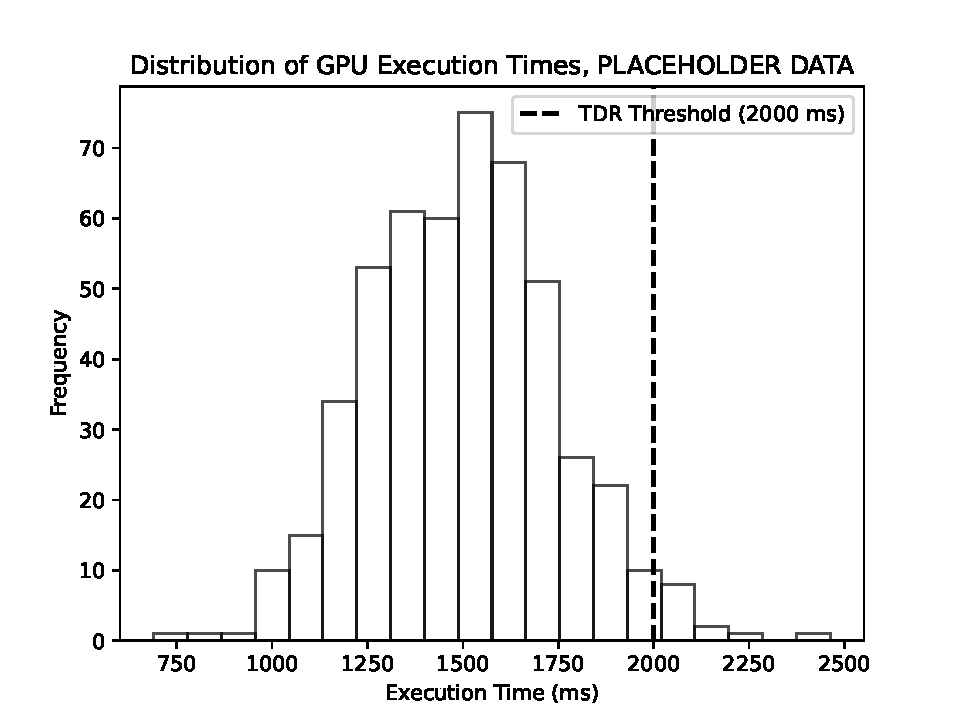
\includegraphics[width=\linewidth]{graphics/Figure_1.pdf}
  \caption{Execution times of \emph{Decoupled Lookback (PLACEHOLDER DATA)}}
\end{figure}
Exacerbating this issue, no major graphics API provides a mechanism to query FPG support. This lack of transparency forces developers to design algorithms without knowing whether critical guarantees are available on the target hardware. In shader environments, where cross-platform portability is essential, this uncertainty compels a fallback to older, less efficient strategies like \emph{Reduce-then-Scan}, sacrificing performance for broader compatibility.

\subsection{Earlier Attempts at Portability}
Our first attempt \raph{we'll add the cite post-review} at implementing a \emph{Decoupled Lookback} scan without relying on FPG was \emph{Scalar Fallback}. Each time a workgroup spins waiting on the reduction from a preceding tile, it advances a \emph{fallback} operation by processing one scalar element from that tile. This eliminates the possibility of deadlock because the number of such operations is bounded; the wait will eventually terminate, possibly at the expense of doing redundant work.

\emph{Scalar Fallback} suffers from two primary inefficiencies. First, the fallback reduction is performed serially by a single thread, progressing only when the lookback thread performs a waiting spin. This results in a $t$-sized blocking tile requiring $t$ spins to complete. Second, once the fallback completes, the lookback thread does not post its result to device memory, forcing every blocked workgroup to redundantly recompute the fallback. While \emph{Scalar Fallback} achieved speed-of-light performance on hardware with FPG and executed correctly without it, its performance on the latter was inferior to \emph{Reduce-then-Scan}.

\section{Decoupled Fallback}
\emph{Decoupled Fallback} addresses both inefficiencies. Our key advance is to utilize the parallelism available in the workgroup to perform the fallback computation, rather than performing it sequentially. To do so requires nontrivial coordination within the workgroup, given that the \emph{Chained Propagation} logic is typically performed by the first thread.

\begin{algorithm}
  \small
  \SetAlgoLined%
  \KwGlobalIn{%
    $\textit{in}[]$,
    $\textit{out}[]$,
    $\textit{spine}[]$,
    $\textit{tileBump}$,
  }
  \KwSharedIn{%
    $\textit{wg\_partials}[]$,
    $\textit{wg\_fallback}[]$,
    $\textit{wg\_prev\_reduction}$,
    $\textit{wg\_broadcast}$,
    $\textit{wg\_control}$,
  }
  \KwGlobalOut{$\textit{out}[]$ inclusive scan of $\textit{in}[]$}
  \KwConstants{Vectors per thread $\textit{p}$}

  \If{$\textit{threadid} = 0$}{
    $\textit{wg\_broadcast} \gets \textnormal{atomicAdd}(\&\textit{tileBump}, 1)$\;
    $\textit{wg\_control} \gets \textnormal{LOCKED}$\;
  }
  \textbf{workgroupBarrier()}\;

  $\textit{tile\_id} \gets \textit{wg\_broadcast}$\;

  $\textit{local\_vectors} \gets \textnormal{array}\langle \textnormal{vec4}\langle u32\rangle, \textit{p} \rangle$\;

  \textbf{Load}($\textit{in}$, $\textit{tile\_id}$, \textit{local\_vectors})\;
  \textbf{SubgroupRake}($\textit{local\_vectors}$, $\textit{wg\_partials}$)\;
  \textbf{workgroupBarrier()}\;

  \textbf{WorkgroupWideScan}($\textit{wg\_partials}$)\;
  \textbf{workgroupBarrier()}\;

  \tcp{Chained Propagation, Decoupled Fallback}
  \textbf{PostLocalReduction}($\textit{spine}$, $\textit{tile\_id}$, $\textit{wg\_partials}$)\;
  \While{$\textit{wg\_control} = \textnormal{LOCKED}$}{
    \textbf{Lookback}($\textit{spine}$, $\textit{tile\_id}$, $\textit{wg\_prev\_reduction}$, $\textit{wg\_control}$)\;
    \textbf{workgroupBarrier()}\;

    \If{$\textit{wg\_control} = \textnormal{LOCKED}$}{
      \textbf{FallbackReduce}($\textit{in}$, $\textit{wg\_fallback}$)\;
      \textbf{FallbackInsertionAttempt}($\textit{spine}$, $\textit{wg\_fallback}$, $\textit{wg\_prev\_reduction}$, $\textit{wg\_control}$)\;
      \textbf{workgroupBarrier()}\;
    }
  }

  \textbf{Write}($\textit{out}$, $\textit{tile\_id}$, $\textit{local\_vectors}$, $\textit{wg\_partials}$, $\textit{wg\_prev\_reduction}$)\;

  \caption{High-Level Scan Kernel}
\end{algorithm}

To optimize the fallback operation, we employ three strategies. (1) First, a shared memory \emph{control flag} enables threads performing the lookback to signal the entire workgroup when a fallback is necessary. (2) Next, we limit the number of spins a thread can perform while waiting on a tile; exceeding this threshold triggers a fallback. While this approach risks \emph{false positive} fallbacks---since a late tile is indistinguishable from a genuinely blocking one---the maximum spin count can be tuned to minimize redundant fallbacks. Increasing the spin count lowers false positives but delays progress in true-blocking scenarios. False positives not only increase memory traffic but also consume compute resources that could be scheduled on the same multiprocessor. (3) After completing a fallback, the workgroup attempts to post the reduction result of the blocking tile, preventing redundant fallbacks by subsequent workgroups.

The viability of \emph{Decoupled Fallback} relies on the same cache locality properties as \emph{Decoupled Lookback}. Since no subgroup scheduler is perfectly fair, all hardware inherently has a natural fallback rate $f$\!, independent of FPG, due to false-positive fallback operations. As a result, memory bandwidth usage increases (and we expect throughput to decrease) by $O(fn)$ to $O((2 + f)n)$. However, just as serial ordering confines spine memory accesses within an $o$-width sliding window, scan input accesses are likewise constrained to an $ot$-width window, increasing their likelihood of residing in cache. As we later empirically demonstrate in Section~\ref{sec:Sim-Blocking}, this cache residency significantly reduces memory access costs, making fallback operations predominantly compute-bound when reducing a blocking tile. Since pure reduction has minimal overhead, throughput approaches $O(2n)$ on most devices.

\section{Implementation}
At a high level, our algorithm follows a five-phase construction:
\begin{enumerate}
  \item[(0)] \textbf {Initialization}: The first thread in the workgroup atomically acquires its work-tile by atomically incrementing a value in global memory.
  \item \textbf{Load Phase}: Each thread loads $p$ vectors, consuming the input in a subgroup-blocked ordering. For a subgroup size $s$ and vector size $v$, each subgroup processes a contiguous block of size $s \cdot p \cdot v$.
  \item \textbf{Subgroup-Rake}: Each thread scans its vectors privately, then joins $p$ raking Kogge-Stone~\cite{5009159} subgroup scans,
        allowing the subgroup-block scan to remain barrier-free and in registers. The subgroup-block reduction is then posted to shared memory. For a workgroup of size $w$, subgroup-raking reduces the size of the local spine to $w/s$.
  \item \textbf{Workgroup-Wide Scan}: The workgroup collectively performs a scan across the subgroup partial reductions, writing the results back to shared memory upon completion.
  \item \textbf{Chained Propagation, Decoupled Fallback}: The local reduction is posted to global memory. Then, the first subgroup in the workgroup performs a lookback operation to acquire the reduction result of all previous workgroups, engaging in fallback operations as necessary. Once completed, this subgroup posts the results to shared memory for the workgroup to consume.
  \item \textbf{Write Phase}: Each subgroup incorporates the results from the workgroup-wide scan and lookback operation to produce and write out the correct output.
\end{enumerate}
Phase 0 ensures that the work tiles are consumed in serial order. Phases 1, 2, 3, and 5 comprise the intra-workgroup scan, following a \emph{Scan-then-Propagate} strategy. Phase 4, \emph{Decoupled Fallback}, is responsible for managing all inter-workgroup dependencies. As our loading and writing phase are typical of scan kernels, we focus here on our portability-specific adaptations.

\begin{algorithm}
  \small
  \SetAlgoLined
  \KwSharedIn{ Array of subgroup partial reductions $\textit{x}$ }
  \KwSharedOut{ Inclusive-scanned $\textit{x}$ }
  \KwConstants{ Workgroup Size $\textit{W}$, Subgroup Size $\textit{S}$ }

  $\textit{spine\_length} \gets \textit{W} / \textit{S}$\;
  $\textit{alignment} \gets 1 << \text{divRoundUp}(\log_2(\textit{spine\_length}), \log_2(\textit{S})) \cdot \log_2(\textit{S})$\;

  $\textit{stride} \gets 1$\;
  $\textit{top\_offset} \gets 0$\;

  \ForEach{$\textit{thread\_id}$ \textbf{in} $\textit{W}$ \textbf{in parallel}}{
    \For{$\textit{j} \gets \textit{S}$ \KwTo $\textit{alignment}$ \textbf{with} $\textit{j} \gets \textit{j} \cdot \textit{S}$}{
      \tcp{Brent-Kung Upsweep}

      $\textit{step} \gets \textit{spine\_length} / \textit{stride}$\;

      \If{$\textit{thread\_id} < \textit{step}$}{
        $\textit{temp} \gets \text{subgroupInclusiveScan}(\textit{x}[\textit{thread\_id} + \textit{top\_offset}])$\;
        $\textit{x}[\textit{thread\_id} + \textit{top\_offset}] \gets \textit{temp}$\;
        \If{$\text{\normalfont highestRankLane}(\textit{thread\_id})$}{
          $\textit{x}[(\textit{thread\_id} / \textit{S}) + \textit{step} + \textit{top\_offset}] \gets \textit{temp}$\;
        }
      }

      \textbf{workgroupBarrier()}\;

      \tcp{Fanout}

      \If{$\textit{j} \neq \textit{S}$}{
        $\textit{reduced\_stride} \gets \textit{j} / \textit{stride}$\;
        $\textit{fanout\_index} \gets \textit{thread\_id} + \textit{reduced\_stride}$\;

        $\textit{cond1} \gets \textit{fanout\_index} < \textit{spine\_length}$\;
        $\textit{cond2} \gets (\textit{fanout\_index} \,\&\, (\textit{j} - 1)) \geq \textit{reduced\_stride}$\;

        \If{$\textit{cond1} \textbf{ \&\& } \textit{cond2}$}{
          $\textit{x}[\textit{fanout\_index}] \gets \textit{x}[\textit{fanout\_index}] + \textit{x}[((\textit{fanout\_index} / \textit{stride}) + \textit{top\_offset}) - 1]$\;
        }
      }
      $\textit{stride} \gets \textit{stride} \cdot \textit{S}$\;
      $\textit{top\_offset} \gets \textit{top\_offset} + \textit{step}$\;
    }
    \textbf{barrier()}\;
  }
  \Return{$\textit{x}$}\;
  \caption{Workgroup-Wide Scan.\label{alg:example}}
\end{algorithm}

\subsection{Workgroup-Wide Scan}
The WebGPU specification supports subgroup sizes $s$, where $s = 2^k$ and $k \in [2, 7]$; on some hardware, subgroup sizes can vary between kernel launches. To handle this variability, we use a generalized radix-$s$ Ladner-Fischer~\cite{10.1145/322217.322232} scan network embedded with Kogge-Stone~\cite{5009159} subgroup scans to perform the scan across the local spine. Because the upsweep phase of the Ladner-Fischer network follows a Brent-Kung~\cite{1675982} construction, assuming shared memory bank width equal to the subgroup size, any subgroup scans beyond the first will experience maximum $s$-way bank conflicts. To mitigate this, we employ a Merrill-Grimshaw~\cite[Section 3.3.5]{Merrill2009} style conflict avoidance strategy, which reduces bank conflicts to the radix base of the network—in our case, $s$. Counterintuitively, the resulting $s$-way conflict differs from the conflicts incurred by the Brent-Kung construction. Rather than multiple threads accessing different indices in the same memory bank, this conflict arises from a fanout originating from a single index. However, such access is interpreted by the hardware as a subgroup \emph{broadcast} operation, resulting in no conflicts. Although the Merrill-Grimshaw avoidance doubles our shared memory requirements, this increase causes no performance degradation due to our modest overall use of shared memory, such as our deliberate retention of vectors in registers and the efficiency of subgroup raking. Thus, this network offers several advantages: minimal depth of $\log_2 n$; asymptotically optimal $O(n)$ size; and zero bank conflicts across all supported subgroup sizes.\footnote{We may also obtain a workgroup-wide reduce operation by omitting the fanout operation and substituting the subgroup Kogge-Stone scan with a subgroup butterfly reduction.\john{I don't get this footnote. ``May also''? What are we actually doing? What's the point of this footnote?}}

\subsection{Decoupled Fallback}
To reiterate, the goal of \emph{Chained Propagation} is twofold: first, to determine the reduction of all preceding work tiles, and second, to relay those values to succeeding tiles to accelerate their own lookback operations. Following the \emph{Decoupled Lookback} technique, we model the inter-workgroup spine as a finite-state machine, where each work tile is represented by a reduction value and a state, stored in global memory. Each tile may exist in one of three states:
\begin{itemize}
  \item \textbf{Not Ready}: The tile has not yet been processed or written to global memory.
  \item \textbf{Ready}: The tile has completed its local reduction and posted it to global memory.
  \item \textbf{Inclusive}: The tile has completed its lookback and updated its posting to reflect the inclusive reduction.
\end{itemize}
Workgroups operate independently; each is responsible for updating its own tile state but may also opportunistically update preceding tiles in the event of a fallback. Tile states transition in a strictly forward direction---\emph{Not Ready} $\rightarrow$ \emph{Ready} $\rightarrow$ \emph{Inclusive}---and never revert. Before kernel launch, all tiles are initialized to \emph{Not Ready} with reduction values set to $\varepsilon$. State transitions imply an update of the reduction value: a transition to \emph{Ready} results in the posting of the local workgroup reduction, and to \emph{Inclusive}, the reduction of all previous workgroup reductions. To coordinate this process across the workgroup, each workgroup initializes a shared memory \emph{control flag} during partition index acquisition. This flag governs both the initiation of fallback operations and the entry and exit of the entire \emph{Decoupled Fallback} phase, which begins immediately after the workgroup-wide scan over partial reductions is completed.

We now detail the \emph{Decoupled Fallback} procedure, presenting the algorithm from the perspective of a single workgroup. The details of tile state encoding and atomic updates are discussed in the following section and may vary depending on the data type, so for simplicity, we describe the operation as being performed by the \emph{first thread} of the workgroup:
\begin{figure}
  \centering
  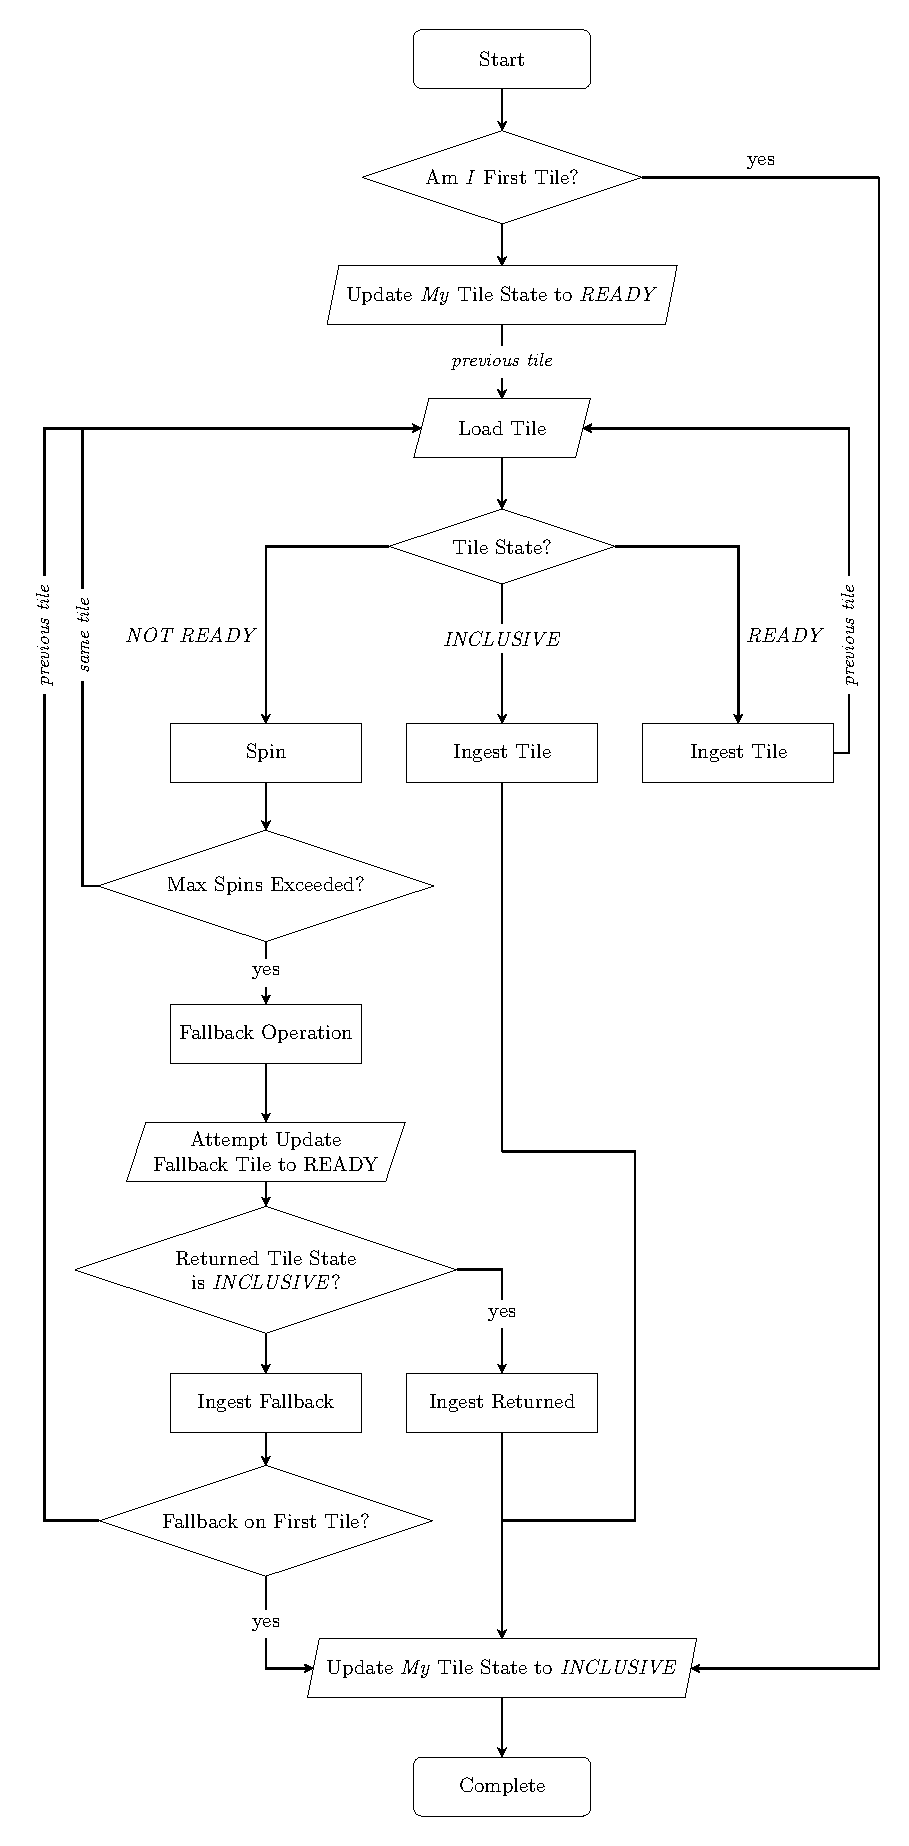
\includegraphics[height=\textheight]{graphics/FlowChart.pdf}
  \caption{Flow Chart Representation of Decoupled Fallback.\label{fig:decoupled_fallback}}
\end{figure}
\begin{enumerate}
  \item[(0)] \textbf{Posting Local Reduction:}
        \begin{itemize}
          \item Each workgroup posts its local reduction---the result of the workgroup-wide scan over partials---to global memory and updates its tile state to \emph{Ready}.
          \item If it is the first work tile, its local reduction \emph{is} its inclusive reduction. In this case, the workgroup updates its tile state directly to \emph{Inclusive} and bypasses the \emph{Chained Propagation} phase entirely.
        \end{itemize}

  \item \textbf{Initialization:}
        \begin{itemize}
          \item The control flag, initialized to \emph{Locked}, signals that the workgroup should enter the \emph{Chained Propagation} phase.
          \item The first thread initializes a \emph{previous reduction} variable in registers with $\varepsilon$ to hold the accumulated reductions of preceding tiles.
          \item The first thread initializes a \emph{current tile} pointer to its immediate predecessor, with which it begins to traverse backwards through the spine.
        \end{itemize}

  \item \textbf{Lookback:}
        \begin{itemize}
          \item The first thread queries the state of \emph{current tile}.
                \begin{itemize}
                  \item If the tile is in the \emph{Ready} state, the workgroup ingests the value and sets \emph{current tile} to the preceding tile, repeating this step until reaching a tile that is \emph{Not Ready}.
                  \item If the tile is in the \emph{Inclusive} state, the workgroup ingests the value and proceeds directly to step~4.
                  \item If the tile is in the \emph{Not Ready} state, the first thread spins for a limited number of iterations, defined by the \emph{Maximum Spin Count}.
                        \begin{itemize}
                          \item If this count is exceeded, it exits the lookback loop and proceeds to step~3, leaving the control flag \emph{Locked} to signal to the workgroup that a fallback is required. Additionally, it copies \emph{current tile} into shared memory to broadcast the fallback tile identity to the workgroup.
                          \item Otherwise, it continues spinning until the tile transitions to a \emph{Ready} or \emph{Inclusive} state. Without FPG, \emph{Decoupled Lookback} risks spinning indefinitely and deadlocking at this stage.
                        \end{itemize}
                \end{itemize}
        \end{itemize}

  \item \textbf{Fallback:}
        \begin{itemize}
          \item If the blocking tile is still \emph{Not Ready} after waiting, the workgroup initiates a fallback operation.
          \item Using the tile index provided by the first thread, the full workgroup computes the reduction of the blocking tile by directly processing the corresponding elements. This process involves a \emph{workgroup-wide reduction},\footnote{See footnote NUMBER.} utilizing additional shared memory to aggregate partial subgroup results.
          \item Once the fallback reduction is complete, the workgroup \emph{attempts} to post the reduction to global memory and update the tile's state to \emph{Ready}.
          \item As this update attempt is performed atomically, the workgroup simultaneously reads back the blocking tile's most recent state:
                \begin{itemize}
                  \item If that most recent state is \emph{Inclusive}, the fallback value computed by the workgroup is discarded, and the first thread ingests the returned value before proceeding to step 4.
                  \item Otherwise, the first thread ingests the fallback value.
                        \begin{itemize}
                          \item If the blocking tile is the first in the spine, the workgroup has reached the start of the spine and has thus completed the \emph{Chained Propagation}. The first thread proceeds to step 4.
                          \item Otherwise, the first thread updates \emph{current tile} to the preceding tile, returning to the lookback process in step~2.
                        \end{itemize}
                \end{itemize}
        \end{itemize}

  \item \textbf{Finalization:}
        \begin{itemize}
          \item To prioritize inter-workgroup reduction propagation, the first thread immediately adds the local reduction to \emph{previous reduction}, posts the inclusive reduction to global memory, and transitions the tile state to \emph{Inclusive}.
          \item It then writes \emph{previous reduction} to shared memory, allowing all threads to combine it with their \emph{workgroup-wide} and private scan computations.
          \item Finally, the first thread sets the control flag to \emph{Unlocked}, signaling the rest of the workgroup that \emph{Chained Propagation} has completed, and allowing the final write phase to begin.
        \end{itemize}
\end{enumerate}

\subsection{Tile State Implementation}
In all variants of \emph{Chained Scan}, there is communication and synchronization between workgroups. The fundamental primitive is \emph{message passing,} meaning that one workgroup posts the result of a communication, then other workgroups read it. This primitive is well-studied in the context of memory models~\cite{Alglave0, MCMutants}. The key requirements here are both control synchronization (meaning the reader does not proceed until the writer sends the message) and data synchronization (meaning that the reader reads the correct value). The latter is especially challenging in relaxed memory models as are employed on GPUs.

Combined control and data synchronization can be accomplished by packing both the tile state and the reduced value into a single word, using relaxed atomic store to send the message, and relaxed atomic load to receive the message, spinning as necessary until the tile state is updated. The semantics of atomics guarantee, even with relaxed memory ordering, that the data is fresh. However, if the tile state and data are stored in separate memory locations, relaxed atomics are insufficient because the compiler is free to reorder stores, so one update does not imply the other. On CPUs, it is common to upgrade the memory semantics from relaxed to acquire/release, which then provides the necessary guarantee~\cite[Section 10.2]{intel_sdm_2024}. Unfortunately, on GPUs, acquire/release semantics are neither portable (they are only available on Vulkan, and optional until version 1.3), nor are they necessarily efficient even when they are available; often the implementation involves expensive cache flushes. A device-scoped memory barrier has similar problems. While it would provide the necessary guarantee, it is also not available in WebGPU (or in versions of Metal prior to 3.2), and is expensive.

Without some other mechanism, the requirement to pack tile state and data into a single word limits the data to 30 bits (assuming 2 bits for the tile state). That, in turn, makes it impossible to represent ordinary 32-bit floating point values without loss of precision. While some GPUs support 64 bit atomics (and it is likely that WebGPU will someday include them as an optional extension), that is also sadly not portable, and merely raises the payload limit to 62 bits without eliminating it altogether.

A key innovation of this paper is to \emph{split} the reduced values into multiple atomics, each carrying its own copy of the tile state. The message is received when relaxed atomic loads of all the parts agree on their tile state. This way, the payload is reconstructed intact, even in the absence of any guarantees from the memory model stronger than relaxed atomics.

\begin{figure}[h!]
  \centering
  \includegraphics[width=\linewidth]{graphics/split.pdf}
  \caption{Splitting one 32-bit value into two 32-bit values with bit-packed tile state.}
\end{figure}

In particular, we use two or four 32-bit values, splitting the reduction value into 16-bit segments while reserving the two most significant bits of each 32-bit value to encode the tile state. Although this could also be accomplished with shared memory (and workgroup barriers), as an optimization, we use two or four threads from the first subgroup, leveraging subgroup \emph{ballot} to verify state consistency, and subgroup \emph{shuffle} to join and split reductions. With one thread per 16 bits and a minimum subgroup size of four in WebGPU, this method supports both 32-bit and 64-bit values, enabling 64-bit scans without 64-bit atomics or memory barriers.\footnote{Although native 64-bit values are not currently supported by the WebGPU specification, their future inclusion is anticipated.}

Fallbacks require a tile state representation and an atomic operation that can safely transition a tile to \emph{Ready} without overwriting a more advanced state. When an update attempt is made, a blocking tile may be in any of the three states due to either of two scenarios: (1) a false-positive fallback on a tile that transitions to \emph{Ready} or \emph{Inclusive} before fallback completion, or (2) another workgroup completing its fallback first, leaving the tile in \emph{Ready}. If the tile state is \emph{Inclusive} then the write must be skipped, especially because races in writes for the parts may leave the tile permanently in an unreadable state. Thus, a simple atomic store is not suitable. An atomic compare-and-swap would have the correct semantics, but WebGPU lacks this primitive (it does have \texttt{atomicCompareExchangeWeak}, which could possibly be made to work but makes reasoning about correctness and performance more difficult). Instead, we encode the tile state in the most significant bits of the atomic value and enforce a strict state ordering: \emph{Inclusive} $>$ \emph{Ready} $>$ \emph{Not Ready}. This allows an \texttt{atomicMaximum}, which successfully updates to a more advanced state but prevents a state regression, to correctly perform updates.

The atomic splitting technique generalizes to monoids of arbitrary size.

\section{Evaluation}
\subsection{Experimental Setup}
We configure workgroups with a size $w = 256$ threads, where each thread processes $p = 4$ vectors of size 4, resulting in 16 elements per thread and a total work tile size of $t = 4096$. We find a maximum spin count of 4 effectively balances responsiveness to blocking while minimizing false-positive fallbacks. As the size of the local spine is inversely proportional to the subgroup size, we allocate sufficient shared memory to accommodate the WebGPU standard's minimum subgroup size of 4. Due to our overall thriftiness with shared memory, total usage remains modest at only $\sim$1 KB\@. For all tests, we use an input size of $2^{25}$ and an inclusive prefix sum. Our test hardware, listed POSITIONAL-RELATION\john{what is $\leftarrow$ POSITIONAL-RELATION\@? Reference the table!}, spans a wide range of FPG and performance capabilities. We empirically find that Google Chrome's native implementation of WebGPU, Dawn, provides the best performance and use it for all testing, except on the Arm-Mali GPU, which requires Android native, necessitating the use of WGPU\@.\footnote{To keep the performance as close to Dawn as possible, we translate our WGSL code with Dawn's Tint transpiler, and provide the raw SPIR-V to WGPU\@.}
\begin{table}
  \centering
  \begin{tabular}{l l c r r}
    \toprule
    Vendor & Device Name            & LOBE         & Occupancy & Subgroup Size \\
    \midrule
    Intel  & HD Graphics 620        & \textbf{Yes} & 9         & 8--32         \\
    ARM    & Mali-G78 MP20          & \textbf{No}  & 40        & 16            \\
    Apple  & M3     (10 Cores)      & \textbf{No}  & 80        & 32            \\
    Apple  & M1 Max (32 Cores)      & \textbf{No}  & 160       & 32            \\
    NVIDIA & GeForce RTX 2080 Super & \textbf{Yes} & 192       & 32            \\
    AMD    & Radeon RX 7900 XT      & \textbf{Yes} & 420       & 32--64        \\
    \bottomrule
  \end{tabular}
  \caption{Hardware Specifications of Testing Devices.\label{tab:hardware}}
\end{table}

\subsection{Performance Comparison}
\subsubsection{Cross-API Performance Versus Contemporary Implementations}
We first compare \emph{Decoupled Fallback} (\emph{DF}) to two key benchmarks: \emph{Memcpy}\textdagger{~\ref{sec:memcpy}} and the \emph{Decoupled Lookback} (\emph{DL}) implementation found in NVIDIA’s CUB library, using the 2080 Super only. To isolate the impact of differing APIs, we implement and evaluate \emph{DF} in both CUDA and Dawn.\footnote{Due to WebGPU’s 128~MB storage buffer limit, our maximum test size is limited to $2^{25}$ 32-bit elements.} \emph{Memcpy} serves as a performance reference, as it shares the same $2n$ global memory movement as \emph{DF} but lacks compute overhead and is purely memory bandwidth bound.

Cross-API comparisons remain challenging, as our CUDA implementation consistently outperforms its Dawn counterpart despite near-identical high-level implementations. The performance cost of \emph{DF} is most pronounced in CUDA when the entire input fits within the 2080 Super’s 4~MB L2 cache, where reduced global memory latency exposes \emph{DF's} increased synchronization and compute overhead compared to CUB\@. However, at larger input sizes, where memory accesses exceed cache capacity, \emph{DF} reaches parity with CUB and achieves \emph{Memcpy} speeds.

\begin{figure}
  \centering
  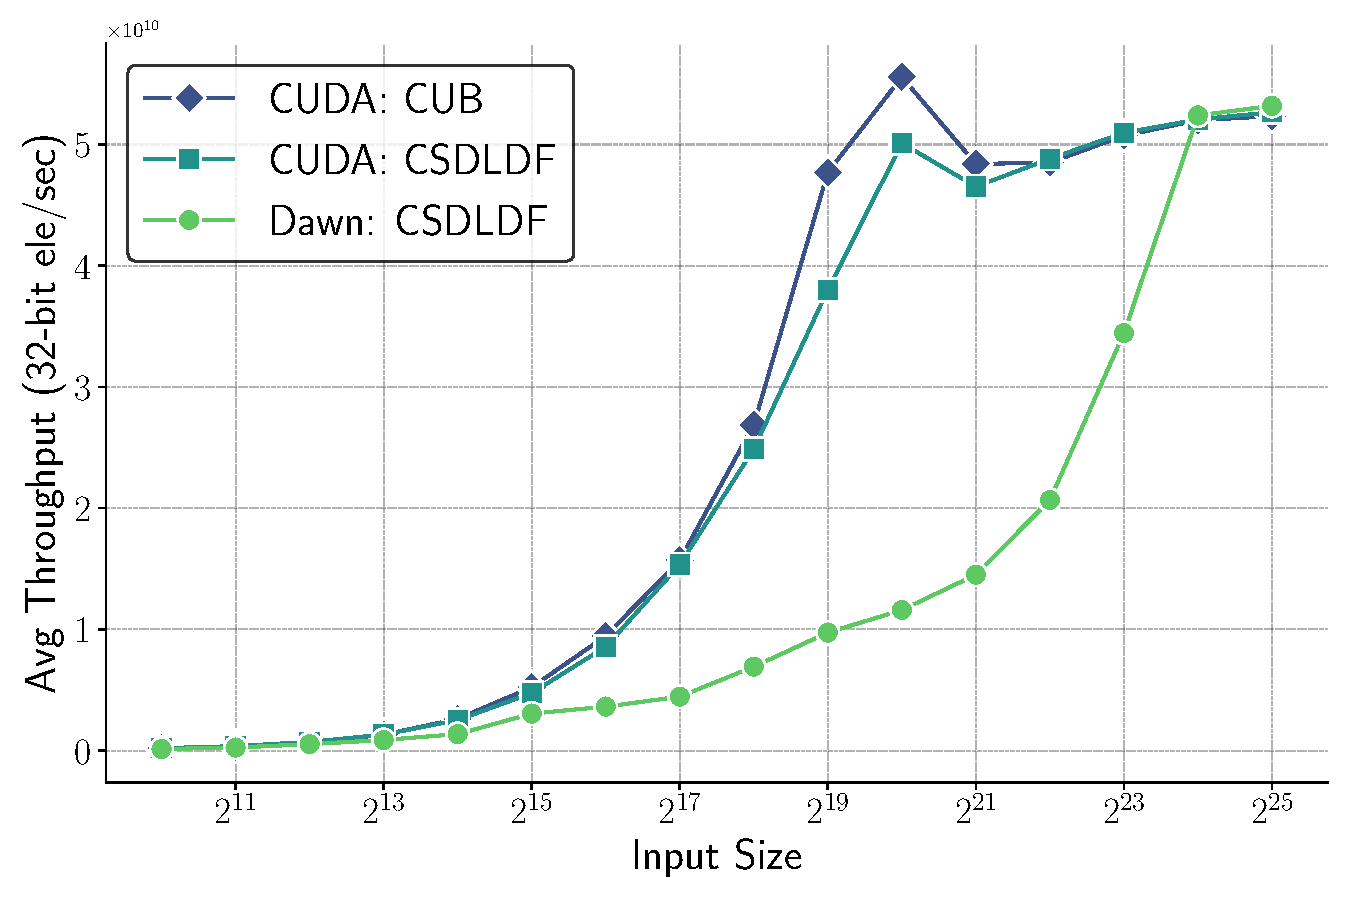
\includegraphics[width=\linewidth]{graphics/cuda_plot.pdf}
  \caption{Performance versus CUB (NVIDIA 2080 Super)}
\end{figure}

\subsubsection{Same-API Performance Versus Baseline Measures}
We next compare \emph{DF} against \emph{Reduce-then-Scan}\textdagger{~\ref{sec:rts}} (\emph{RTS}), which serves as a baseline to highlight the performance improvements of our approach over the prior FPG-constrained technique. This evaluation is conducted using Dawn across the full range of tested devices.

\begin{table*}
  \centering
  \small
  \setlength{\tabcolsep}{1pt}
  \begin{tabular*}{\textwidth}{@{\extracolsep{\fill}} l r r r r r r}
    \toprule
    Metric & \!\!\!\!\!\!Intel HD620 & ARM Mali-G78 MP20 & Apple M3 & Apple M1 Max & Nvidia 2080 Super & AMD 7900 XT \\
    \midrule
    Avg \emph{Memcpy} (32-bit ele/sec $\cdot 10^9$)  & 1.50   & 2.48  & 10.25  & 38.62  & 54.39  & 72.28  \\
    Avg \emph{DF} (32-bit ele/sec $\cdot 10^9$)   & 1.49   & 2.79  & 10.22  & 38.84  & 53.29  & 94.60  \\
    Avg \emph{RTS} (32-bit ele/sec $\cdot 10^9$)      & 1.06   & 2.02  & 6.81   & 25.13  & 35.90  & 61.49  \\
    \emph{DF}/\emph{Memcpy}       & 99.1\%    & 112.8\%  & 99.8\%    & 100.6\%   & 98.0\%    & 130.9\%   \\
    \emph{DF}/\emph{RTS}          & 140.2\%   & 138.5\%  & 150.2\%   & 154.5\%   & 148.4\%   & 153.8\%   \\
    Avg Spins per workgroup    & 0.305    & 1.477    & 0.606    & 0.604    & 0.419    & 0.148    \\
    Avg Lookback Length per workgroup& 1.726    & 3.537    & 3.415    & 10.782   & 13.046   & 20.722   \\
    Avg Total Fallbacks Initiated      & 254.662   & 2504.704  & 365.546   & 990.962   & 86.400   & 9.308   \\
    Avg Total Successful Insertions    & 6.170     & 122.436   & 4.612     & 0.012    & 0.284    & 0.020    \\
    \bottomrule
  \end{tabular*}
  \caption{\emph{Decoupled Fallback} performance, 32-bit Inclusive Prefix Sum, $\mathbf{2^{25}}$ 32-bit elements.\label{tab:results}}
\end{table*}

As shown in Table~\ref{tab:results}, \emph{DF} achieves at least a $\sim$40\% speedup over \emph{RTS} across all tested devices, closely approaching the theoretically expected $O(3n)/O(2n)$ 50\% speedup, except on the ARM Mali. \emph{DF} closely matches \emph{Memcpy} across most devices, deviating only on the AMD 7900 XT and ARM Mali, where \emph{DF} outperforms \emph{Memcpy} by 30.9\% and 12.8\%, respectively. This suggests that additional compute latency may mitigate paging effects by separating loads from stores. On the ARM Mali, \emph{DF} appears to underperform, achieving only a 36\% speedup instead of the expected 50\%. However, its nearly identical performance to \emph{Memcpy} indicates that the implementation is memory-bandwidth-bound, limiting further gains.

\subsection{Decoupled Fallback Statistics}
To better understand how devices interact with \emph{DF}, we collect the following statistics during its execution: \john{Below, I advocate that we say, for each of the four bullets, what we expect / what would be a good result / what the hardware actually does in practice. The reader doesn't deeply know what to expect / what is good.}
\begin{itemize}
  \item \textbf{Spins per Workgroup:} How many times does a workgroup make a waiting spin?
  \item \textbf{Lookback Length per Workgroup:} How many work tiles does a workgroup traverse to complete \emph{Chained Propagation}? \john{Example for above point: something like ``We hope that even with unfair hardware schedulers, this traversal is short (only a few tiles), but we also want to ensure that DF is robust and delivers good performance for even long traversals.''}
  \item \textbf{Total Fallbacks Initiated:} What is the total number of fallback operations initiated across all workgroups?
  \item \textbf{Total Successful Insertions:} What is the total number of fallback operations that successfully update a blocking (or late) tile to \emph{Ready}?
\end{itemize}
Despite differing occupancy rates, the number of waiting spins remains consistent across devices. \john{Is this a small number? Large? Tell don't show.} Likewise, lookback length is stable and remains well below the theoretical occupancy bound. Expressed as a percentage of occupancy, it remains under 10\% for all devices, except for the Intel HD620, where its elevated value is likely an artifact of its low absolute occupancy. Most notably, the devices lacking FPG---Apple M3 and M1 Max---do not exhibit significantly higher successful insertion rates than the others, suggesting that true deadlocking is a rare occurrence.

\subsection{Simulated Blocking}%
\label{sec:Sim-Blocking}
To demonstrate the resilience of our technique to unfair schedulers, we simulate fallback rates significantly higher than those observed organically by intentionally omitting work tile reduction updates. Because these updates are skipped, the immediate successor workgroup reads \emph{Not Ready}, spinning and triggering a fallback. Starting with infrequent omissions---1 in 512 work tiles---we progressively increase the omission rate to near-continuous levels---1 in 2 work tiles---recording \emph{DF} statistics at each step.
\begin{figure*}
  \centering
  \begin{subfigure}[t]{0.48\linewidth}
    \centering
    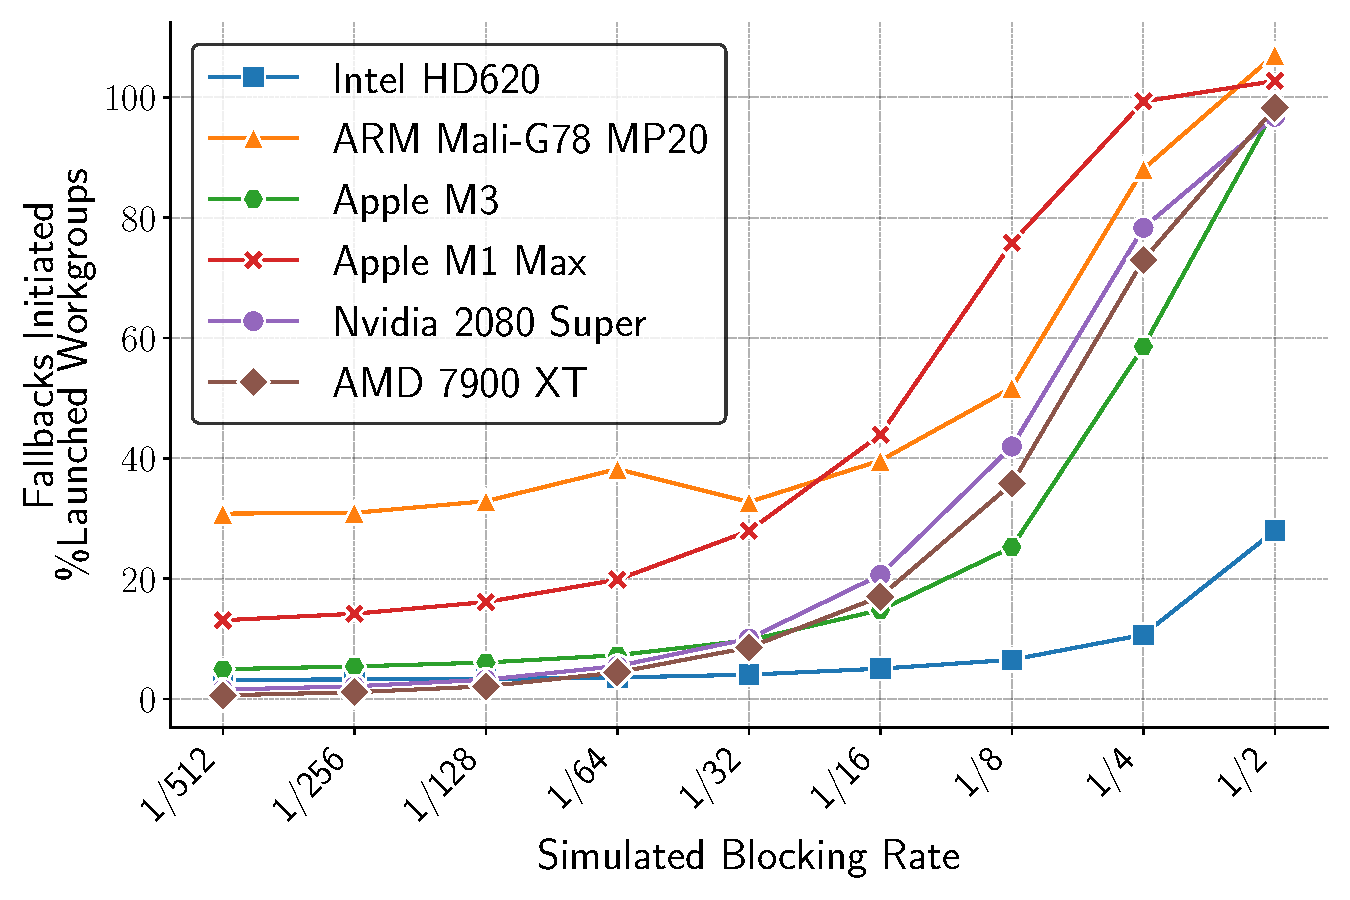
\includegraphics[width=\linewidth]{graphics/fallbacksInitiated_plot.pdf}
    \caption{Fallbacks Initiated.\label{fig:fallbacks_initiated}}
  \end{subfigure}\hfill
  \begin{subfigure}[t]{0.48\linewidth}
    \centering
    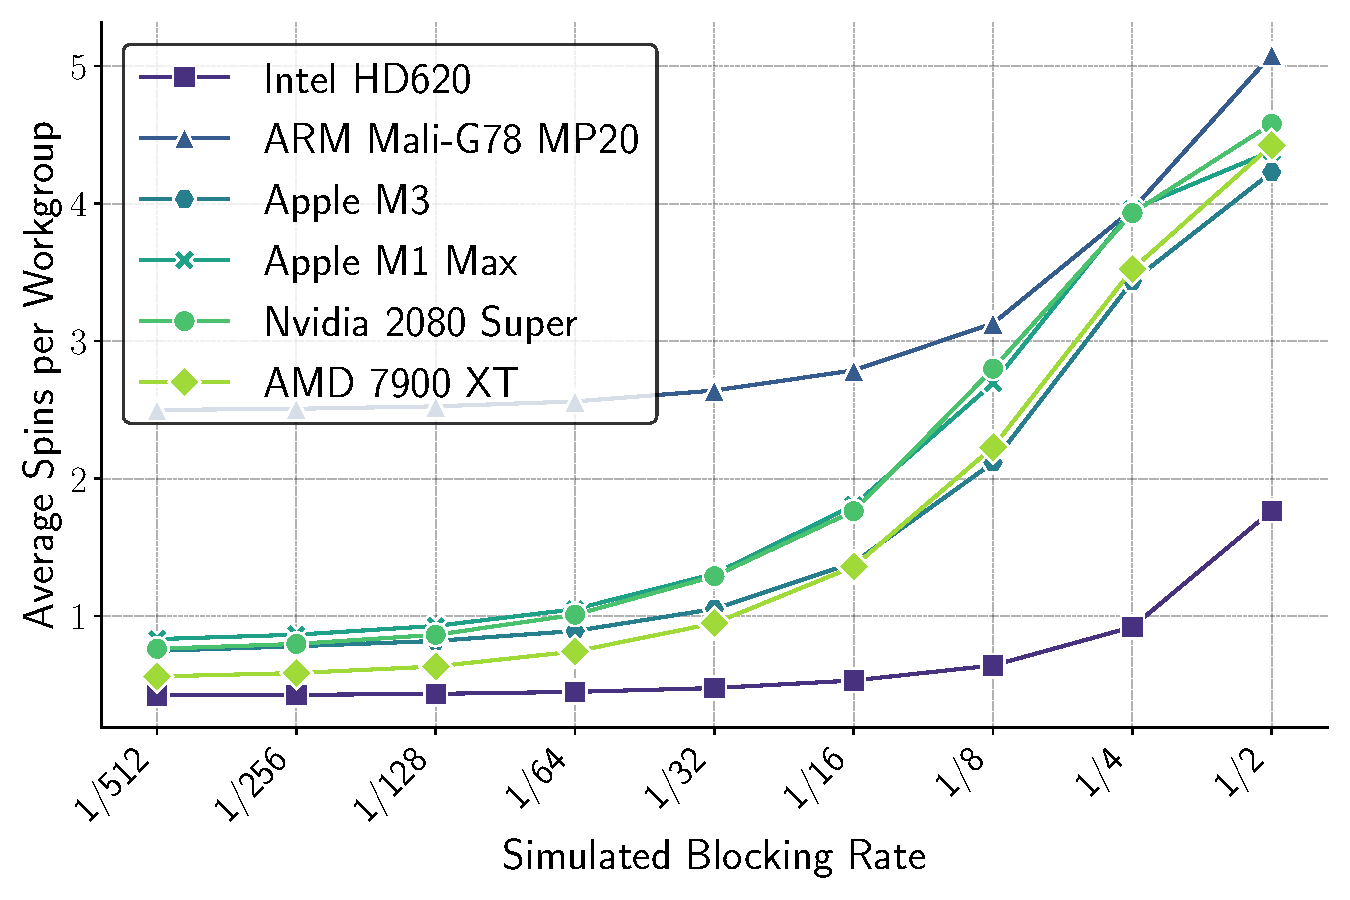
\includegraphics[width=\linewidth]{graphics/totalSpins_plot.pdf}
    \caption{Total Spins.\label{fig:total_spins}}
  \end{subfigure}

  \vspace{0.2em}

  \begin{subfigure}[t]{0.48\linewidth}
    \centering
    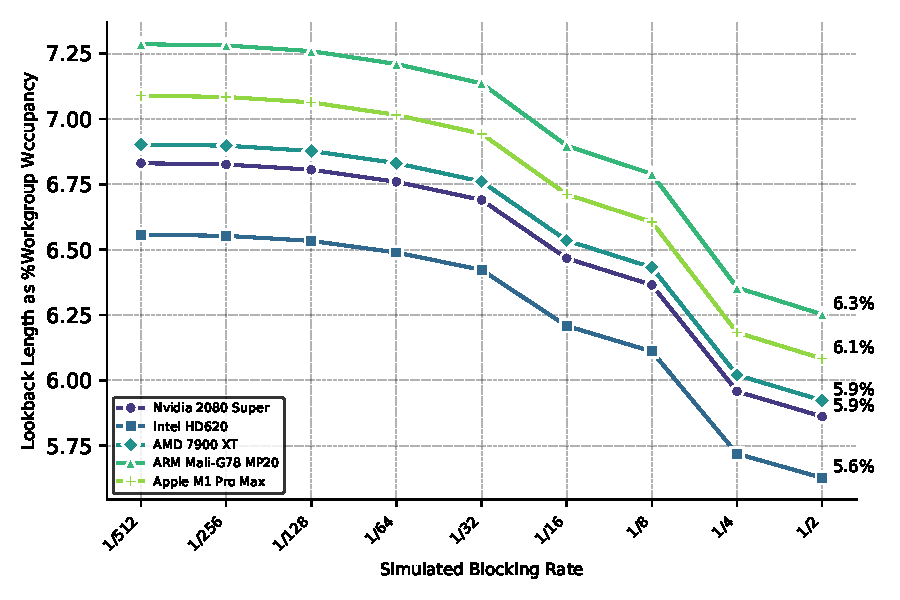
\includegraphics[width=\linewidth]{graphics/lookbackLength_plot.pdf}
    \caption{Lookback Length.\label{fig:lookback_length}}
  \end{subfigure}\hfill
  \begin{subfigure}[t]{0.48\linewidth}
    \centering
    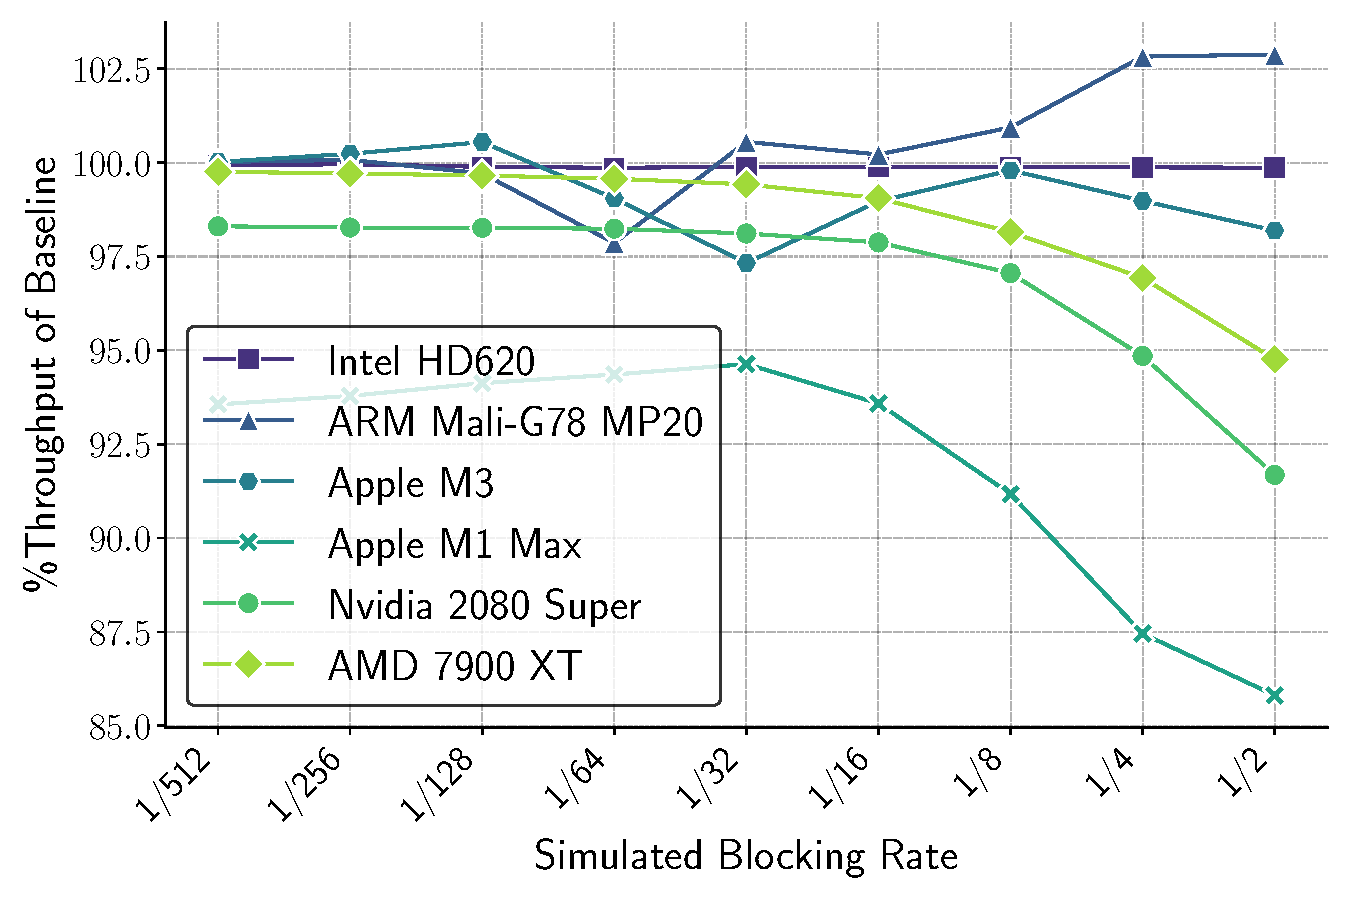
\includegraphics[width=\linewidth]{graphics/time_plot.pdf}
    \caption{Throughput vs.\ Baseline.\label{fig:execution_time}}
  \end{subfigure}

  \caption{Simulated Blocking. \john{Please write a good caption here---this is an important caption to write! Probably writing subfigure captions is the right way to go (explain each of them individually).}\label{fig:vertical_images}}
\end{figure*}

As shown in Figure~\ref{fig:execution_time}, performance relative to a no-omission baseline remains above 85\% even at near 100\% fallback rates across all devices---except for the Intel HD620, where only a 25\% fallback rate is induced. Notably, this performance level remains well above the equivalent \emph{RTS} performance of 66\%; \emph{DF} is consistently faster than the previous standard for portable scans. While Figures~\ref{fig:fallbacks_initiated} and~\ref{fig:total_spins} confirm that we are inducing fallbacks, this test primarily measures the impact of increasing fallback operations rather than true blocking behavior. The finer details of this distinction are discussed next.
\section{Discussion}

\subsection{Trade-offs}
\emph{Decoupled Fallback} introduces several tradeoffs that must be considered: (1) Without a memory barrier, the scan cannot be performed in place and requires a separate output buffer to prevent false-positive fallback operations on post-scanned values, as the tile state may not update before the scan values. (2) For monoids larger than 64 bits, multiple subgroups are required, increasing synchronization overhead due to the need for shared memory and barriers. (3) In certain in-situ compaction algorithms where fallback work-tiles cannot be easily reduced and must be held in registers, Decoupled Fallback may reduce occupancy. (4) Additionally, in compute-bound in-situ compaction algorithms, the cost of fallbacks may outweigh the savings from reduced global memory traffic. (5) Lastly, because the control flow of \emph{Decoupled Fallback} requires barriers, latency incurred during lookback cannot be hidden by workgroup computation.

\subsection{Limits on Speed-of-Light Performance}
Due to its increased latency, synchronization overhead, and longer critical path, \emph{Decoupled Fallback} exacerbates existing challenges faced by \emph{Decoupled Lookback}, particularly a lack of compute capacity and unfair scheduling. Devices that already lack sufficient compute resources to reach SOL performance are especially affected, as the additional compute overhead from fallback operations cannot be hidden by memory loads and stores. The worst-case scenario arises in devices that suffer from both low compute power and unfair scheduling.

Another potential bottleneck is the speed of atomic operations. On some older GPUs---such as pre-Fermi NVIDIA architectures---atomics do not operate within the cache, resulting in significantly higher latency. Slower atomics lead to delayed tile updates, which in turn increase lookback lengths. While our simulated deadlocks provide an artificial means of stress-testing execution, real deadlocks manifest as an effective \emph{occupancy reduction}: execution resources remain available, but fewer subgroups can context-switch to mitigate latency.

\subsection{Future Work}
Sorting is one of the most notable beneficiaries of single-pass scan and, by extension, \emph{Decoupled Fallback}. The current state-of-the-art algorithm, Adinets and Merrill’s \emph{Onesweep}~\cite{adinets2022onesweepfastersignificantdigit}, is an 8-bit least-significant-digit radix sort, where single-pass scan minimizes data movement during digit-binning passes. However, due to its compute-intensive nature and large $radixDigit$-sized monoid, it is unclear whether \emph{Decoupled Fallback} will map well to sorting or if new techniques are needed.

Our reexamination of \emph{Chained Scan} with dynamic assignment raises fundamental questions about the GPU progress models proposed by Sorensen et al.~\cite{sorensen2021}: Can all HSA algorithms be converted to OBE via dynamic assignment? Are there cases, excluding atomic memory errors, where LOBE guarantees termination but dynamic assignment with OBE does not? Is OBE all you need?

\subsection{Conclusion}
In this paper, we presented \emph{Decoupled Fallback}, a single-pass \emph{Chained Scan} capable of reaching SOL performance under all progress models and suitable for implementation within the constraints of contemporary portable shading languages. Our approach maintains minimal data movement while ensuring robust execution across diverse GPU architectures.

\begin{acks}
\end{acks}

\bibliographystyle{ACM-Reference-Format}
\bibliography{bib}

\clearpage
\appendix
\section{Artifact}
\subsection{Availability}
We provide our artifact in the following GitHub repository: \thomas{Will anonymize with GithubAnonymous once we are ready}. The repository contains per API requirements and building instructions.

\subsection{Baseline Comparisons: \emph{Memcpy}}%
\label{sec:memcpy}
\begin{table}
  \small
  \centering
  \begin{tabular}{l r r}
    \toprule
    Device                                & \makecell{Memory           \\ Bandwidth \\ (GB/s)} & \makecell{Expected \\ Throughput \\ (32-bit ele/sec)} \\
    \midrule
    Intel HD620 Single-Channel            & 17.1             & 2.13e9  \\
    Intel HD620 Dual-Channel              & 34.1             & 4.26e9  \\
    ARM Mali-G78 MP20 / Tensor (Pixel 6a) & 51.2             & 6.40e9  \\
    Apple M3 (10 Cores)                   & 102.4            & 12.8e9  \\
    Apple M1 Max (32 Cores)               & 409.6            & 51.2e9  \\
    Nvidia 2080 Super                     & 496              & 62.0e9  \\
    AMD 7900 XT                           & 800              & 100.0e9 \\
    \bottomrule
  \end{tabular}
  \caption{Vendor-Specified Memory Bandwidth and Expected Throughput (32-bit Elements per Second).\label{tab:memory_bandwidth}}
\end{table}
Although all of Dawn's backend APIs support \emph{timestamp queries inside encoders}, Apple GPUs do not, so we are forced to implement our own \emph{Memcpy} kernel to measure memory bandwidth, as opposed to simply timing an API's copy buffer operation. It is well known that \emph{observed} peak memory bandwidth tends to diverge from vendor-listed peak bandwidth, so for completeness we list these figures above. We make a number of observations:
\begin{itemize}
  \item \textbf{Intel HD620:} As our HD620 laptop is only equipped with a single memory DIMM, its peak bandwidth is limited to the lower bound, 2.13e9 ele/sec. Thus, our observed bandwidth of 1.498e9 is reasonable.
  \item \textbf{ARM Mali-G78 MP20 / Pixel 6a (Tensor):} The observed throughput is significantly lower than expected, despite a vendor-listed bandwidth of 6.40e9 ele/sec. The cause of this discrepancy remains unclear, but we note other developers have observed similar speeds.
  \item \textbf{Apple M1 Pro Max:} Observed throughput matches expectations.
  \item \textbf{Nvidia 2080 Super:} Observed throughput matches expectations.
  \item \textbf{AMD 7900 XT:} Our above result, where \emph{DF} was observed to be faster than \emph{Memcpy}, is likely due to compute latency counterintuitively improving memory access patterns, leading to reduced paging. Furthermore, we see that our \emph{DF} throughput is within spec and reasonable.
\end{itemize}

\subsection{Baseline Comparisons: \emph{Reduce-then-Scan}}
\label{sec:rts}
As we desire the most competitive baseline possible, our \emph{RTS} kernels employ the same intra-workgroup scan strategy and tuning parameters as \emph{DF}. Initially, we adopted Merrill and Grimshaw's~\cite{Merrill2009} workgroup raking approach for inter-workgroup processing. However, empirical testing revealed that raking was consistently outperformed—by up to $\sim$15\% on lower-end devices—by a simpler approach that processes the spine serially with a single workgroup. Furthermore, our \emph{RTS} performance closely aligns with the theoretically expected $O(3n)$ global memory movement.

\end{document}
\endinput

%%% Local Variables:
%%% mode: LaTeX
%%% TeX-master: t
%%% End:
